\documentclass[]{article}

%opening
\title{4F13 Probabilistic Machine Learning - Latent Dirichlet Allocation}
\author{Candidate: 5562E}

%packages
\usepackage[margin=0.5in]{geometry}
\usepackage[export]{adjustbox}
\usepackage{graphicx}
\usepackage{amsmath}
\usepackage{amssymb}
\usepackage{hyperref}
\usepackage{caption}
\usepackage{subcaption}
\usepackage{parskip}
\usepackage{listings}
\usepackage{pdfpages}
\usepackage{bbm}

%package setup
\graphicspath{{./img/}}
\DeclareMathOperator*{\argmax}{arg\,max}
\DeclareMathOperator*{\argmin}{arg\,min}

%custom commands
\newcommand{\Fcal}{\mathcal{F}}
\newcommand{\idft}{\mathcal{F}^{-1}}
\newcommand{\Xcal}{\mathcal{X}}
\newcommand{\Ncal}{\mathcal{N}}
\newcommand{\Acal}{\mathcal{A}}
\newcommand{\Bcal}{\mathcal{B}}
\newcommand{\cmplx}{\mathbb{C}}
\newcommand{\Lcal}{\mathcal{L}}
\newcommand{\Mcal}{\mathcal{M}}
\newcommand{\indep}{\perp \!\!\! \perp}
\newcommand{\iid}{\stackrel{iid}{\sim}}
\newcommand{\figwidth}{0.6\linewidth}
\newcommand{\betaml}{\hat{\beta}^{ML}}

%section numbering
\renewcommand{\thesubsection}{\alph{subsection}}

\begin{document}

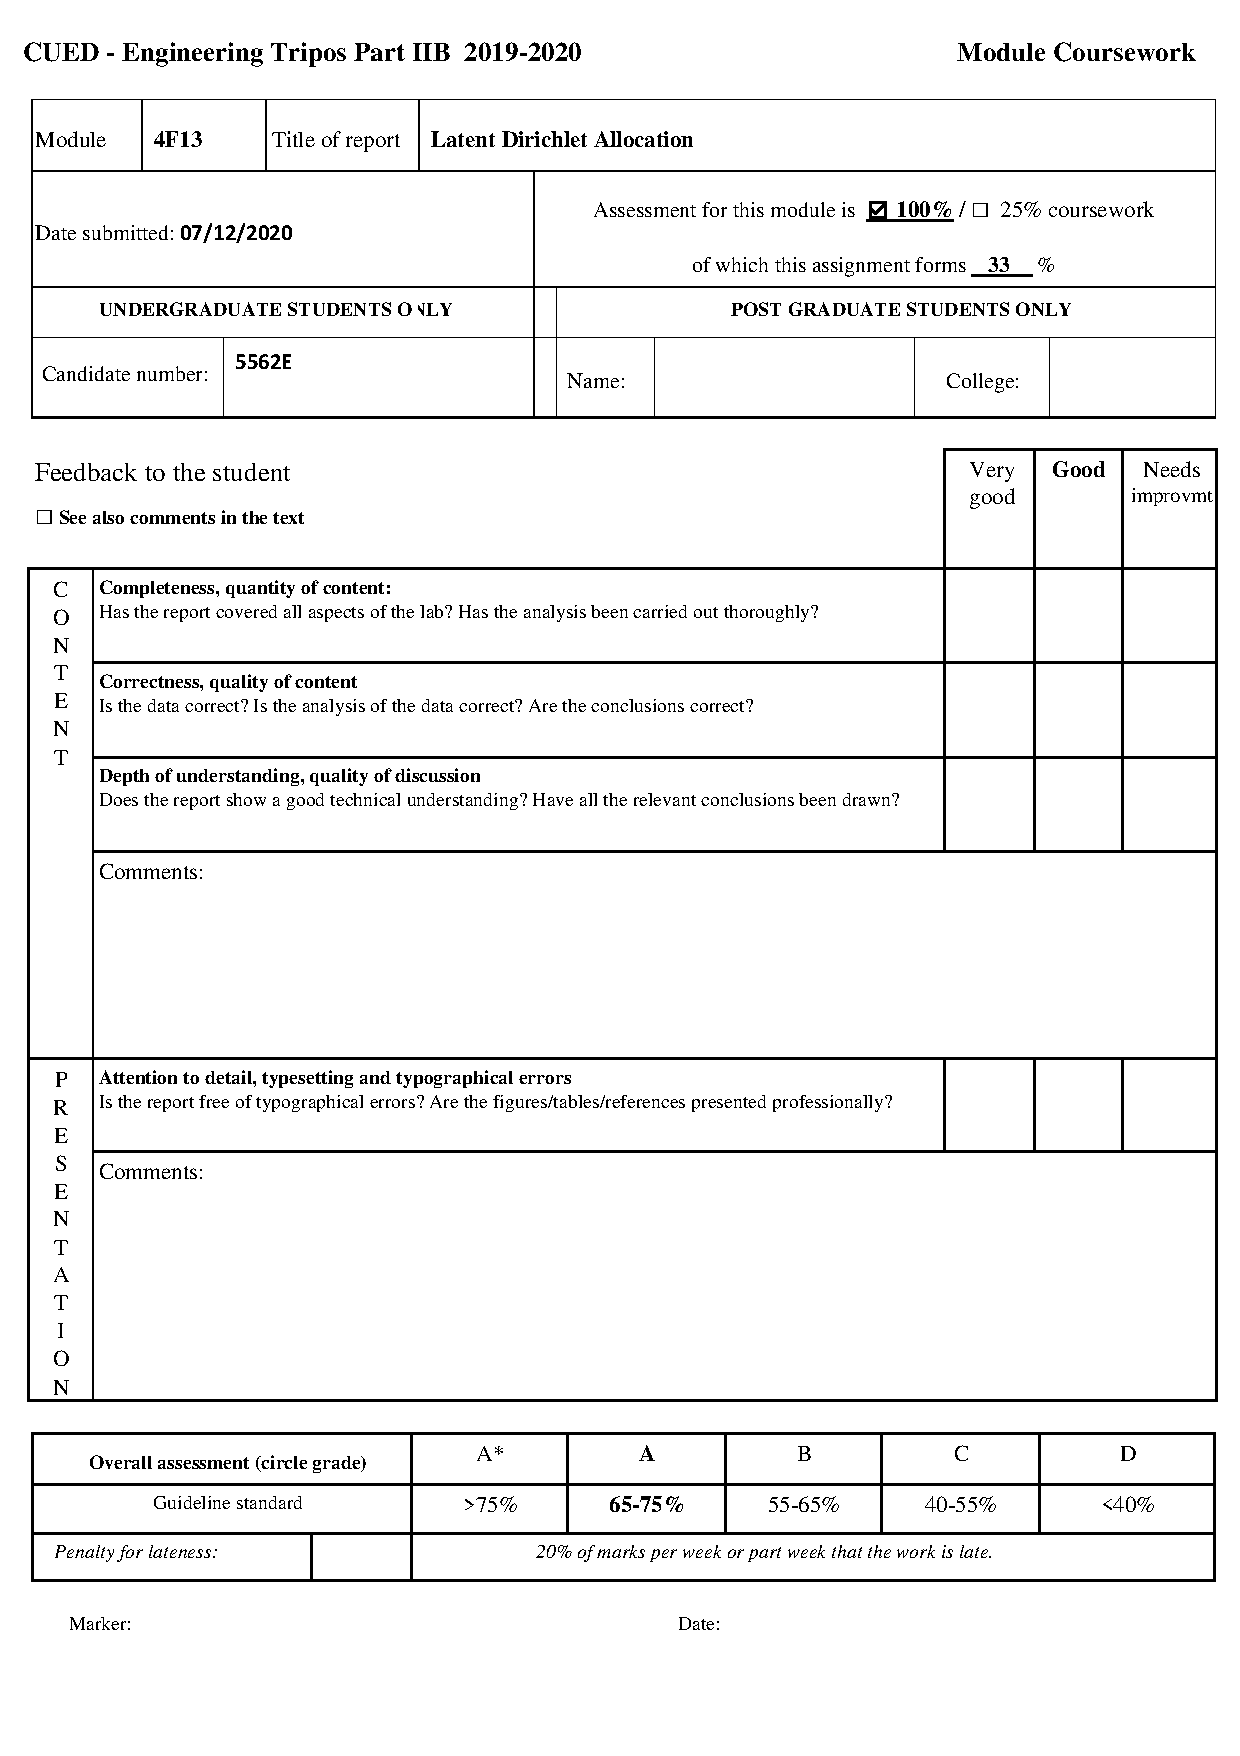
\includepdf[pages={1}]{coversheet-CW3.pdf}

\setcounter{page}{1}
\maketitle

\tableofcontents

\section{Introduction}

We have a document test set $\Acal$, which consists of $D$ documents indexed by $d \in \{1 \dots D\}$. A document is an ordered list of words. The vocabulary $\Mcal$ has $M=|\Mcal|$ unique words. We denote the $n$'th word in the $d$'th document by $w_{nd} \in \{1 \dots N_d\}$. Where $N_d$ is the length of document $d$. For simplicity we denote the count of occurences of word $m$ in the test set by $c_m$.

We hold back a test set $\Bcal$ to calculate the performance of our approaches.

\section{Questions}
\subsection{Maximum Likelihood}

We begin by assuming that each word is drawn independently from a categorical distribution with parameter $\beta$: $w_{nd} \iid Cat(\beta)$. In this case $\beta$ is a $M \times 1$ vector with the conditions that $\sum_{m=1}^{M} \beta_m = 1$ and $\beta_i \geq 0$. The likelihood of the parameter $\beta$ is the probability of the dataset given $\beta$:
%
\begin{equation}
	L(\beta) = P(\Acal | \beta) = \prod_{d=1}^{D} \prod_{n=1}^{N_d} P(w_{nd} | \beta) = \prod_{m \in \Mcal} \beta_m ^{c_m}
\end{equation}
%
Where $c_m$ is the count of word $m$ in the training set. We wish to obtain the Maximum-Likelihood estimate $\betaml = \argmax L(\beta)$. We prefer to maximise the log-likelihood as this is more tractable:
%
\begin{equation}
	\Lcal(\beta) = \log L(\beta) = \sum_{m \in \Mcal} c_m \log \beta_m
\end{equation}
%
We can now take derivatives and include a Lagrange multiplier to respect the sum to 1 constraint:
%
\begin{equation*}
	\frac{\partial}{\partial \beta_i}  \left\{ \Lcal(\beta) + \lambda \left(1 - \sum_{m=1}^{M} \beta_m \right) \right\}_{\beta = \betaml} = \frac{c_i}{\betaml_i} - \lambda= 0
\end{equation*}
\begin{equation}
	\therefore \betaml_i = \frac{c_i}{\lambda} = \frac{c_i}{\sum_{m \in \Mcal} c_m} = \frac{c_i}{C}
\end{equation}
%
Therefore, the ML estimate is simply the empirical frequency of each word (normalised by the sum of all counts $C$).
%
\begin{figure}[!h]
	\centering
	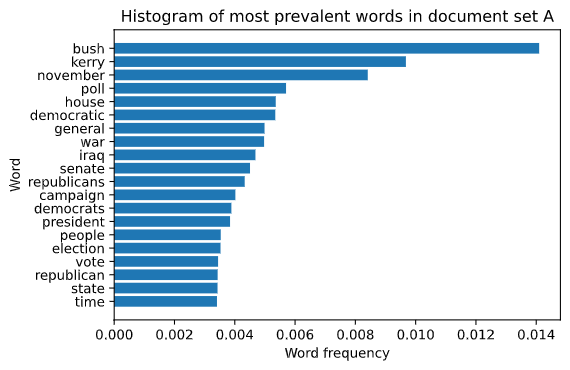
\includegraphics[width=\figwidth]{hist-ml.png}
	\label{fig:hist-ml}
	\caption{Histogram of top 20 most prevalent words in test set A}
\end{figure}
\subsection{Bayesian Inference}

\textbf{Words}: XX

\end{document}
